\chapter{Konzept}
\label{cha:konzept}
Der Aufbau und das Systemdesign des Aktivitäts-Tracking-Frameworks bilden einen zentralen Bestandteil dieser Arbeit. In diesem Kapitel werden die einzelnen Komponenten beschrieben, die für das Tracking von Aktivitätsdaten erforderlich sind. Die praktische Umsetzung des Konzepts erfolgt anschließend in Kapitel \ref{cha:implementierung}.

\section{Systemarchitektur}
Bevor die einzelnen Komponenten im Detail erläutert werden, beschreibt dieser Abschnitt die Zusammenarbeit und die übergeordnete Struktur der Teilbereiche und Systemkomponenten.

\subsection{Komponenten und Aufbau}

\subsubsection{Teilbereiche und Komponenten}
\label{sec:system_design}
Das Tracking-Framework besteht aus sechs Teilbereichen, die gemeinsam den gesamten Funktionsumfang des Systems abdecken.

\begin{itemize}
    \item Systemkonfiguration
    \item Trackingkonfiguration
    \item Daten- und Aktionsermittlung
    \item Filterung und Extraktion
    \item Vermittlung und Ablaufsteuerung
    \item Datenaustausch und Zwischenspeicherung
\end{itemize}

Im Rahmen der Implementierung (siehe Kapitel \ref{cha:implementierung}) wurden diese Teilbereiche in eigenständige Komponenten unterteilt, sodass alle Aufgaben aus diesen Bereichen berücksichtigt werden. Bestimmte Teilbereiche, wie beispielsweise der Datenaustausch und die Zwischenspeicherung, wurden dabei auf mehrere Komponenten verteilt.

\subsubsection{Struktur der Komponenten}
Abbildung \ref{fig:system_design_components} zeigt, wie die einzelnen Komponenten im System zusammenarbeiten. Das zentrale Element bildet der {Tracking-Manager}, über den alle Komponenten miteinander verbunden sind. Jede Komponente verfügt über eine klar definierte Schnittstelle, die den Zugriff ermöglicht. Nur der Tracking-Manager kennt die einzelnen Komponenten, während diese untereinander vollständig entkoppelt und unabhängig voneinander agieren. Die einzige Komponente, die von mehreren Komponenten genutzt wird, ist die Systemkonfiguration. Sie wird vom Tracking-Manager verwaltet und an die jeweiligen Komponenten weitergegeben.

Diese Struktur sorgt für eine hohe Flexibilität. Änderungen, die von der Systemumgebung abhängen, können vorgenommen werden, ohne andere Teile des Frameworks zu beeinflussen. So lässt sich beispielsweise die Art der Datenverarbeitung anpassen, ohne dass der übrige Aufbau geändert werden muss.

\begin{figure}[H]
    \centering
    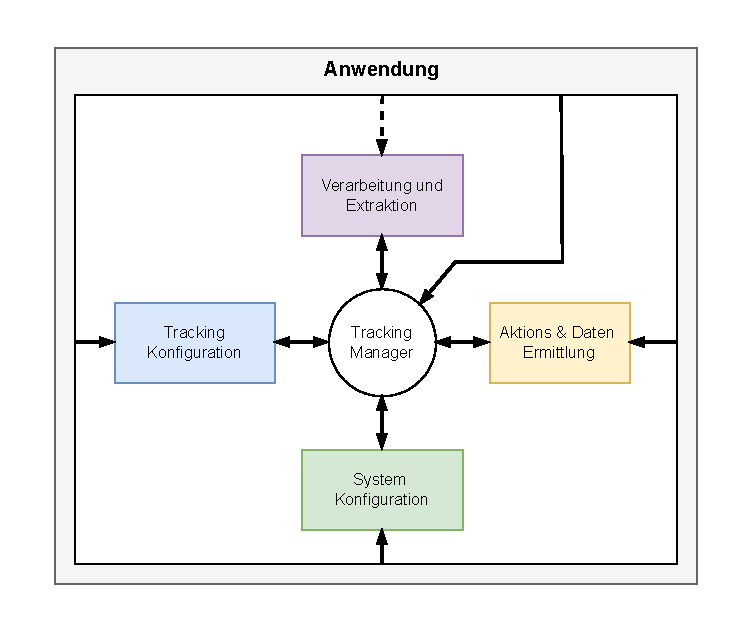
\includegraphics[width=0.65\textwidth]{5_Systemdesign_Components_Tracking}
    \caption{Zusammenhänge der Komponenten im Tracking-Framework.}
    \label{fig:system_design_components}
\end{figure}

Die lose Kopplung besteht nicht nur zwischen den internen Komponenten des Frameworks, sondern auch zwischen der Anwendung und dem Framework selbst. Die Anwendung stellt die Tracking-Konfiguration, Anwendungsdaten sowie eine Systemkonfiguration bereit. Optional kann sie auch Funktionen zum Filtern und Extrahieren übernehmen.
Diese Daten werden über eine definierte Schnittstelle sowie vordefinierte Komponenten und Templates an das Framework übermittelt. Dadurch wird sichergestellt, dass für die Integration nur minimale Kenntnisse über das Framework erforderlich sind. In den meisten Fällen erkennt das Framework seine Abhängigkeiten zur Anwendung selbstständig.

Die Anwendung selbst muss im Wesentlichen lediglich die erforderlichen Daten über eine definierte Schnittstelle bereitstellen. Dadurch lässt sich das System flexibel in unterschiedlichen Technologien einsetzen, beispielsweise in WPF (siehe Unterabschnitt \ref{subsec:WPF}) oder Windows Forms (siehe Unterabschnitt \ref{subsec:Winforms}).

\subsection{Kommunikation zwischen Komponenten}
\label{subsec:communication_between_coponents}

\subsubsection{Kommunikationsgrundlage}
Damit ein Informationsaustausch zwischen den Komponenten möglich ist, wird eine gemeinsame Kommunikationsbasis benötigt. Diese Grundlage besteht aus Objekten, die die gemeinsame Sprache für den Datenaustausch definieren.  
Konzeptionell wird zwischen fünf Informationskategorien unterschieden:

\begin{itemize}
    \item \textbf{Trackingaktionen}: Repräsentieren auftretende Ereignisse innerhalb der Anwendung.
    \item \textbf{Trackingdaten}: Umfassen Daten, die auf Basis einer aufgetretenen Aktion erfasst werden.
    \item \textbf{Extraktionsaufgaben}: Beschreiben, welche Informationen aus Trackingaktionen und Trackingdaten ermittelt werden sollen, und stellen Metadaten für die resultierenden Extraktionsdaten bereit.
    \item \textbf{Trackingaufgaben}: Legen fest, welche Daten für die Weiterverarbeitung ermittelt und verarbeitet werden dürfen.
    \item \textbf{Extraktionsdaten}: Enthalten die aus Trackingaktionen und Trackingdaten extrahierten Informationen, die anschließend weiterverarbeitet oder übermittelt werden können.
\end{itemize}

Die einzelnen Kategorien können verschiedene Objekttypen enthalten, die je nach Anwendungsfall unterschiedlich ausgestaltet sind. Diese Objekte bilden einen grundsätzlich unveränderlichen Standard, wobei Extraktionsdaten, Trackingaktionen und Trackingdaten durch benutzerdefinierte Objekte erweitert werden können. Damit die Daten vom Framework verarbeitet werden können, müssen sie, ähnlich wie bei Google Analytics (siehe Unterabschnitt \ref{subsec:google_analytics}), einer festgelegten Struktur entsprechen.

\subsubsection{Datenübertragungswege}
Der Datenaustausch zwischen den Komponenten kann entweder direkt über Rückgabewerte von Funktionen oder über sogenannte Datenkanäle erfolgen.  
Ein Datenkanal ist im Rahmen dieser Arbeit als ein Konstrukt zu verstehen, über das Daten an eine unbekannte oder externe Komponente weitergegeben werden können.  
Durch die Systemkonfiguration (siehe Abschnitt \ref{sec:integration_concept}) kann die Anwendung verschiedene Wege der Veröffentlichung oder des Bezugs von Daten anbieten. Auf diese Weise bleibt das System flexibel gegenüber unterschiedlichen Datenquellen und Zielen.

\subsubsection{Ablauf der Kommunikation}
Der Ablauf der Kommunikation erfolgt über die zuvor beschriebenen Datenobjekte und wird im in Abbildung \ref{fig:sequence_diagram_communication_components} dargestellten Sequenzdiagramm veranschaulicht.  
Wie dort gezeigt, erzeugt die Anwendung zunächst alle benötigten Komponenten. Die Reihenfolge ergibt sich aus den jeweiligen Abhängigkeiten, wobei die genaue Erstellungsreihenfolge zwischen Datenermittlung (Abschnitt \ref{sec:data_collection_concept}), Verarbeitung (Abschnitt \ref{sec:data_extraction_concept}) und Trackingkonfiguration (Abschnitt \ref{sec:configuration_concept}) nicht entscheidend ist.  

Nach der Erzeugung wird der Tracking-Manager initialisiert. Während dieser Initialisierung wird auch die Systemkonfiguration (siehe Abschnitt \ref{sec:integration_concept}) übergeben. Anschließend initialisiert der Tracking-Manager die Trackingkonfiguration, die wiederum die benötigten Assemblies für die Konfiguration ermittelt. Danach kann der Tracking-Manager die Aufgaben für das Tracking anfordern. Diese Aufgaben werden bei der Initialisierung der Komponenten für Datenermittlung sowie für Verarbeitung und Extraktion berücksichtigt.

\begin{figure}[H]
    \centering
    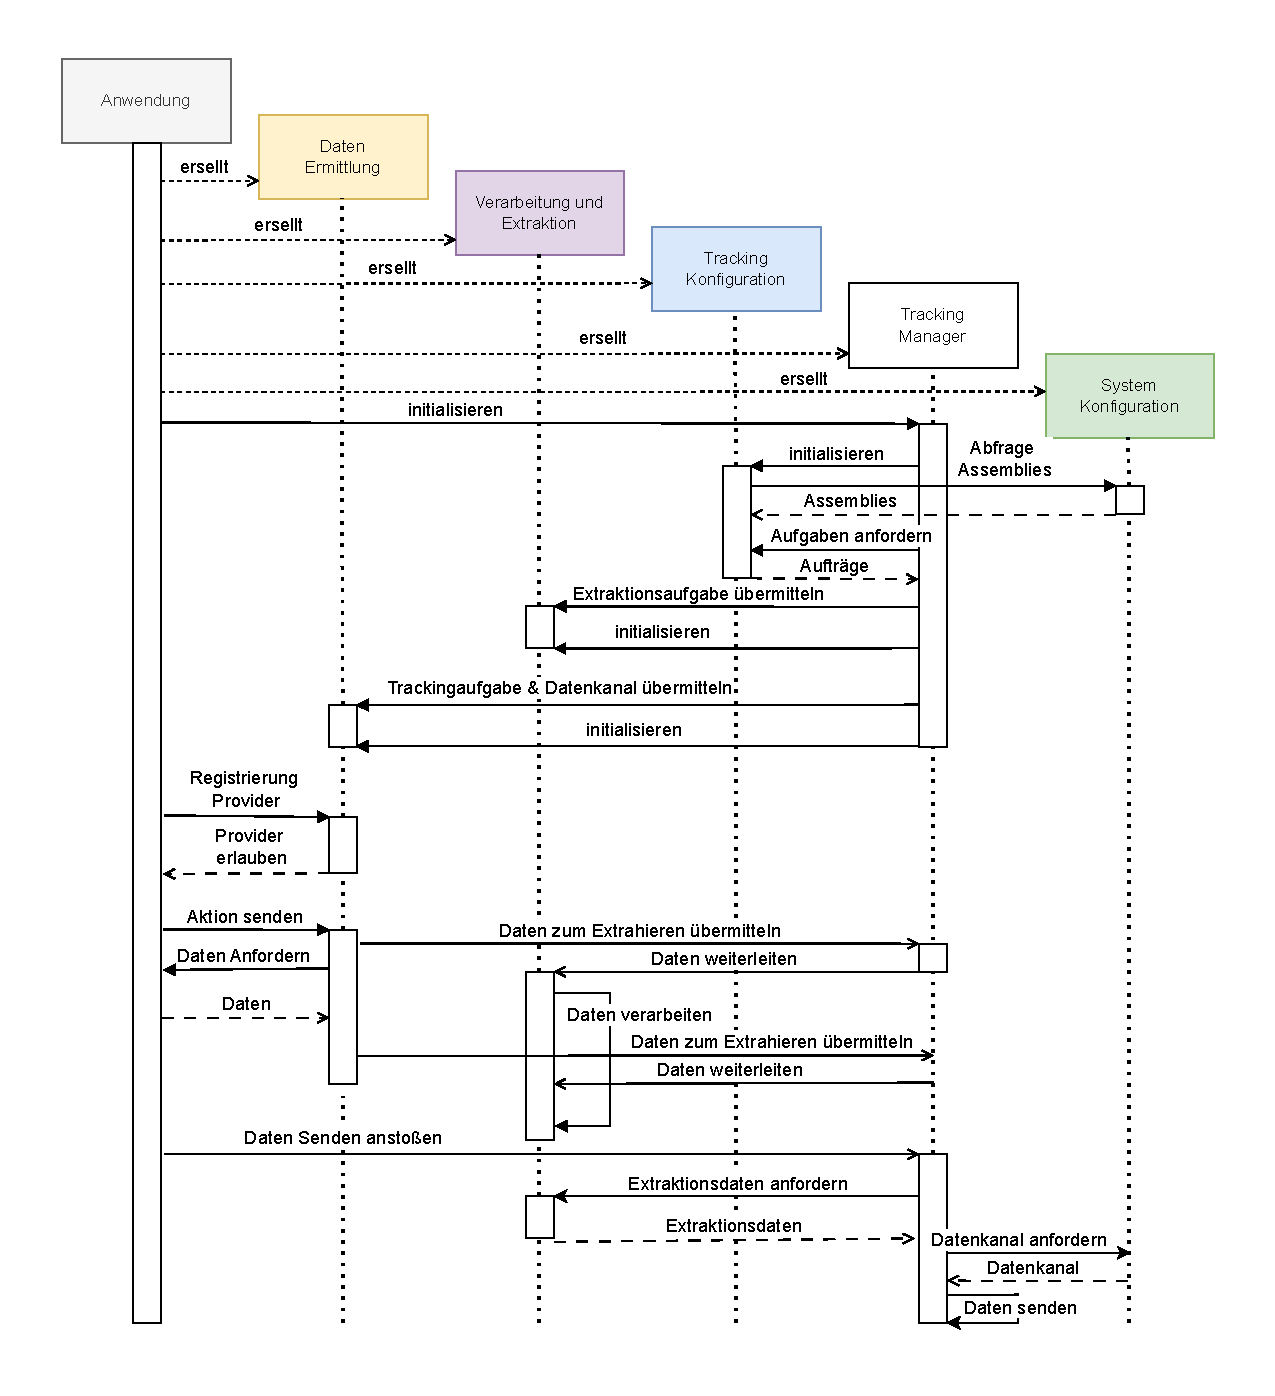
\includegraphics[width=1.0\textwidth]{5_Sequence_Diagram_Components_Communication}
    \caption{Ablauf der Kommunikation zwischen den Komponenten.}
    \label{fig:sequence_diagram_communication_components}
\end{figure}

Nach Abschluss der Initialisierung kann die Anwendung sogenannte Data Provider registrieren. Dabei entscheidet die Komponente zur Datenermittlung, ob ein Provider einen entsprechenden Datenkanal zur Übertragung von Daten erhält. Über diesen Kanal können sowohl Aktivitätsdaten als auch nachgelieferte Daten gesendet werden.

Die übergebenen Daten werden anschließend in der Extraktionskomponente asynchron zur Anwendung empfangen und weiterverarbeitet.  

Wenn die Anwendung das Ausliefern der Daten anstößt, fordert der Tracking-Manager die Extraktionsdaten an und übergibt sie über den in der Systemkonfiguration bereitgestellten Datenkanal an die entsprechende Zielkomponente.

\section{Tracking-Konfiguration}
\label{sec:configuration_concept}
Wie bei Google Analytics (siehe Unterabschnitt \ref{subsec:google_analytics}) und OpenTelemetry (siehe Unterabschnitt \ref{subsec:open_telemetry}) verfügt auch dieses Framework über eine Konfiguration, in der festgelegt wird, welche Daten getrackt werden sollen. Für das hier vorgestellte Framework ist eine hybride Lösung vorgesehen, die sowohl Online-Konfigurationen, wie bei Google Analytics, als auch Code-basierte Konfigurationen, wie bei OpenTelemetry, ermöglicht. In dieser Arbeit wird jedoch ausschließlich die zweite Variante konzipiert und umgesetzt.

\subsection{Aufbau der Konfigurationskomponente}
Der Aufbau der Konfigurationskomponente ist in Abbildung \ref{fig:configuration_component} dargestellt. Diese Komponente besteht aus einem Manager, der sowohl für die Initialisierung als auch für die Bereitstellung der Aufgaben verantwortlich ist. Der Manager agiert dabei als Slave des Hauptmanagers.

Das Erstellen der Konfiguration erfolgt durch sogenannte Configuration Builder, die zuvor über eine Fluent API \footnote{Unter einer Fluent API oder auch einem Fluent Interface \cite{Fowler2005FluentInterface} versteht man eine Methodik des Method-Chaining, bei der Konfigurationen in einer flüssigen, satzähnlichen Syntax formuliert werden können.} definiert werden. Optional soll die Komponente so erweitert werden können, dass künftig auch ein Konfigurationsserver angebunden werden kann. Im Rahmen dieser Arbeit bleibt dies jedoch unberücksichtigt.

\begin{figure}[H]
    \centering
    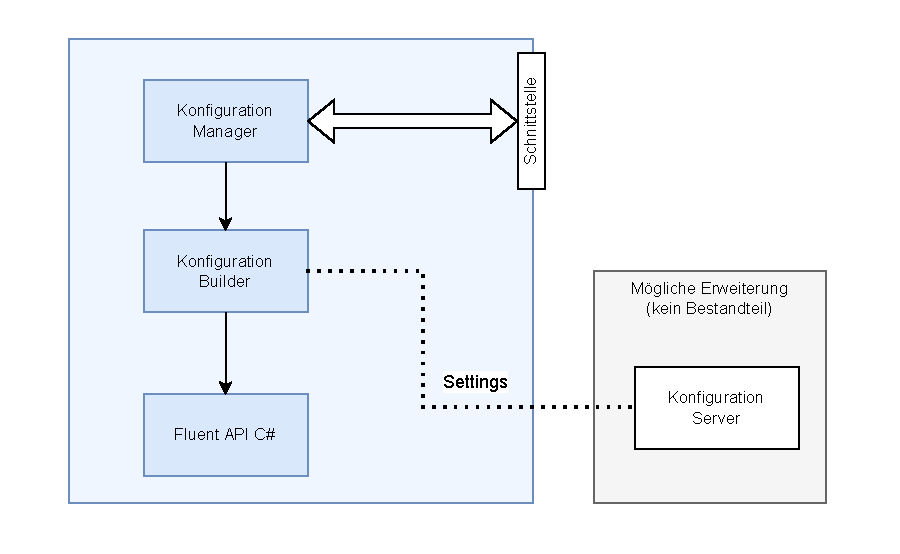
\includegraphics[width=0.55\textwidth]{5_Configuration_Component}
    \caption{Aufbau der Konfigurationskomponente}
    \label{fig:configuration_component}
\end{figure}

\subsection{Konfigurationsmöglichkeiten und Fluent API}

\subsubsection{Kategorien von Informationen}
Um die ursprünglich definierten Fragen (siehe Unterabschnitt \ref{subsec:initial_questions}) beantworten zu können, müssen bestimmte Informationen gesammelt werden. Diese lassen sich in folgende Kategorien einteilen:

\begin{itemize}
    \item \textbf{Metriken:} Zahlenbasierte Daten, wie sie bereits im Zusammenhang mit OpenTelemetry beschrieben wurden. Beispiele hierfür sind die Ladezeit einer Ansicht oder die Anzahl der Öffnungen einer bestimmten Ansicht.
    \item \textbf{Daten:} Informationen, die beispielsweise aus einer Ansicht extrahiert werden können, etwa die Anzahl der Einträge in einer Liste.
    \item \textbf{Nutzung:} Informationen, die Aufschluss über das Nutzungsverhalten der Anwendung geben, beispielsweise wie häufig ein Shortcut in einer bestimmten Ansicht verwendet wird.
    \item \textbf{Workflows:} Informationen, die mit Traces in OpenTelemetry vergleichbar sind und einen Ablauf von aufeinanderfolgenden Aktionen darstellen.
\end{itemize}

\subsubsection{Aufbau der Fluent API}
Die zuvor kategorisierten Daten können weiter beschrieben werden, woraus sich ein Schema ableiten lässt, das für den Aufbau der Fluent API von zentraler Bedeutung ist.\\
\\
$Kontext \rightarrow Kategorie \rightarrow Kategorieoptionen$\\
\\
Daten stammen stets aus einem bestimmten Kontext und gehören zu einer der oben definierten Kategorien. Diese Daten können anschließend durch spezifische Optionen weiter unterteilt werden. Ein vereinfachter Ausschnitt der Fluent API nach diesem Schema wird in Abbildung~\ref{fig:configuration_component_fluent_api} als Syntaxdiagramm dargestellt. Mit der in der Abbildung gezeigten API ist es möglich, das Anfordern von Daten aus einer Ansicht zu konfigurieren.

\begin{figure}[H]
    \centering
    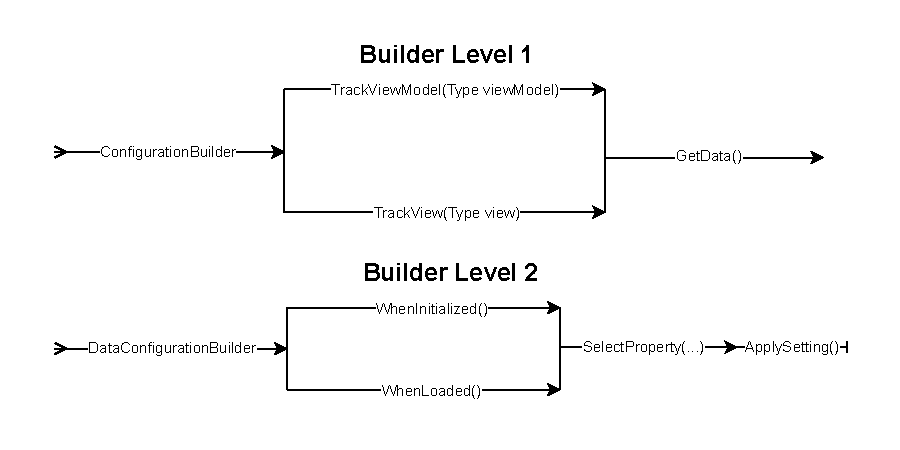
\includegraphics[width=0.82\textwidth]{5_Configuration_Component_Fluent_API}
    \caption{Vereinfachter Ausschnitt der Fluent API für die Tracking-Konfiguration.}
    \label{fig:configuration_component_fluent_api}
\end{figure}

\subsection{Builder und deren Funktionsweise}
Builder \cite{sarcar2004design} sind spezielle Klassen, die konfiguriert werden können und anschließend durch den Aufruf einer Build-Methode entsprechende Objekte erzeugen. Nach der Erzeugung können diese Objekte vom Builder abgerufen werden. Der Director ist die Komponente, die den Erstellungsprozess steuert. Im Kontext dieser Arbeit übernimmt der Manager diese Rolle.

\subsubsection{Bessere Aufgabenteilung durch mehrstufige Builder}
In Abbildung \ref{fig:configuration_component_fluent_api} ist von zwei Builder-Leveln die Rede. Der Grund dafür liegt darin, dass ein einzelner Builder sehr umfangreich und unübersichtlich werden würde. Um die Wartbarkeit und Erweiterbarkeit zu verbessern, werden die Builder daher in mehrere Ebenen unterteilt.  
Der Builder der ersten Ebene ruft die Build Methode der nachfolgenden Ebenen auf und fügt deren Ergebnisse zusammen. Dieses Prinzip folgt dem Composite-Muster \cite{gamma1995design}.

\subsection{Settings und deren Zusammenhang mit Builder}
Aus Sicht der Anwender*innen der API existieren keine Builder direkt. Die Fluent API verwendet stattdessen bestimmte Settings, die am Ende einem Builder hinzugefügt werden. Auf Grundlage dieser Einstellungen kann der Builder anschließend die entsprechenden Objekte erstellen, beispielsweise die Aufgaben zur Datenermittlung (siehe Abschnitt~\ref{sec:data_collection_concept}) und zur Extraktion der Daten (siehe Abschnitt~\ref{sec:data_extraction_concept}).  
Dieser Zusammenhang wird in Abbildung \ref{fig:builder_and_settings_cooperation} dargestellt.

\begin{figure}[H]
    \centering
    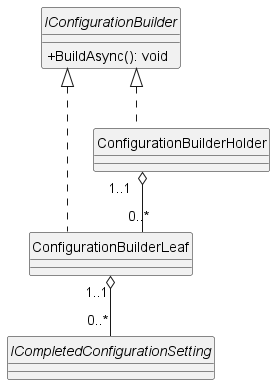
\includegraphics[width=0.4\textwidth]{5_Configuration_Concept_Builder_Class_Diagramm}
    \caption{Klassendiagramm für den Zusammenhang zwischen Builder und Settings.}
    \label{fig:builder_and_settings_cooperation}
\end{figure}

\subsection{Bereitstellen von Einstellungen}
Wie bereits erläutert, werden Einstellungen über eine Fluent-API konfiguriert und einem Builder hinzugefügt. Da Softwaresysteme häufig sehr umfangreich sind, werden sie meist in kleinere Teilprojekte unterteilt. Die in dieser Arbeit behandelte Integration (siehe Kapitel \ref{cha:implementierung}) bezieht sich genau auf ein solches System.

Aus diesem Grund erfolgt die Konfiguration auf Assembly-Basis (siehe Abschnitt \ref{subsec:assemblies}). Konkret bedeutet das, dass pro Assembly mehrere Settings-Provider existieren können, die beim Erstellen einer Konfiguration ausgelesen werden. Diese Provider erhalten eine Starteinstellung (den Einstiegspunkt der Fluent-API) und wenden die entsprechenden Einstellungen automatisch über die API auf einen Builder an.

Diese Provider werden von den Entwickler*innen implementiert, indem die Fluent-API wiederholt auf die jeweilige Starteinstellung angewendet wird. Dabei wird festgelegt, welche Informationen aus dem jeweiligen Teil der Anwendung (der sich in derselben Assembly befinden muss) ermittelt werden sollen.

\section{Daten- und Aktionsermittlung}
\label{sec:data_collection_concept}
Auf Basis der Konfiguration wird, wie bereits beschrieben, ein Tracking-Auftrag erteilt. Dieser Auftrag kann anschließend von der Anwendung abgearbeitet werden. Wie diese Abarbeitung im Detail erfolgt, wird in diesem Abschnitt erläutert.

\subsection{Komponentenstruktur und Aufgabenverteilung}
\label{subsec:data_collection_components}
Abbildung \ref{fig:structure_data_collection} zeigt die Struktur der Daten- und Aktionsermittlungskomponente. Teile dieser Struktur wie die Provider befinden sich innerhalb der Anwendung, während ein Manager die Integration in das Trackingsystem übernimmt. In diesem Unterabschnitt wird dargestellt, welchen Beitrag die einzelnen Bestandteile zur Datenermittlung leisten.

\begin{figure}[H]
\centering
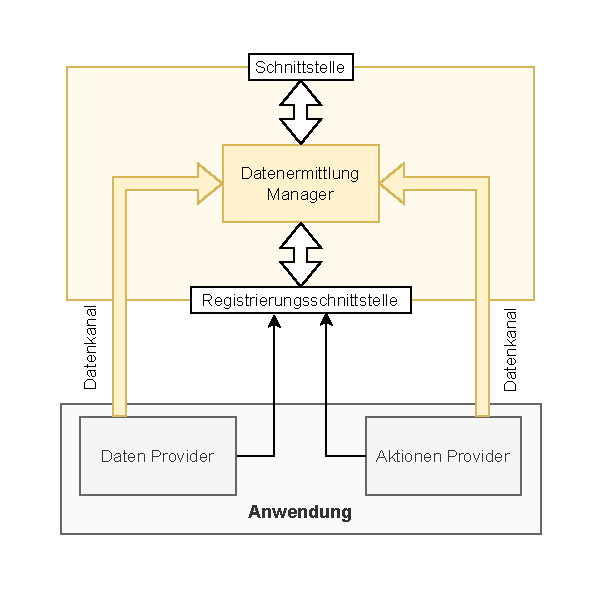
\includegraphics[width=0.52\textwidth]{5_Data_Collection_Structure}
\caption{Struktur der Datenermittlungskomponente.}
\label{fig:structure_data_collection}
\end{figure}

\subsubsection{Manager für Datenermittlung}
Zunächst ist entscheidend, dass in diesem Kontext unter Datenermittlung sowohl die Erfassung von Aktionen als auch der daraus resultierenden Daten verstanden wird. Der Manager übernimmt daher die Aufgabe, die Zugangskontrolle für beide Arten von Providern sicherzustellen. Dabei wird geprüft, ob ein Provider einen Beitrag zum jeweiligen Tracking-Auftrag leisten kann. Ist dies der Fall, bestätigt der Manager die Teilnahme des Providers durch die Bereitstellung eines Datenkanals.

Wenn anschließend Aktionen über diesen Datenkanal übermittelt werden, ist es die Aufgabe des Managers, die entsprechenden DataProvider zu informieren und die Ermittlung der zugehörigen Daten auszulösen.

Der Datenkanal wird vom Manager wiederum an einen übergeordneten Datenkanal weitergeleitet, der vom Hauptmanager bereitgestellt wird. Damit ist der Manager dem Hauptmanager untergeordnet, analog zum Aufbau beim Konfigurationsmanager.

Insgesamt verwaltet der Manager somit die Tracking-Aufträge und stellt sicher, dass diese ordnungsgemäß und vollständig ausgeführt werden, wie in Abbildung \ref{fig:structure_data_collection} dargestellt ist.

\subsubsection{Provider für Aktionen}
Aktionen sind, wie bereits in Unterabschnitt \ref{subsec:communication_between_coponents} beschrieben, ein wesentlicher Bestandteil der Kommunikation von Ereignissen innerhalb der Anwendung. Sie werden von speziellen Action Providern bereitgestellt, sofern dies vom Manager für Datenermittlung vorgesehen ist.

Die Aktionen werden im jeweiligen Provider über eine Fabrikkomponente erzeugt, deren Implementierung je nach System variieren kann. Provider sind nur aktiv, wenn ihre Registrierung beim zugehörigen Manager erfolgreich abgeschlossen wurde.

Die Übergabe der Aktionen erfolgt nach dem Push-Prinzip, um eine asynchrone Weiterverarbeitung und Filterung zu ermöglichen. Dadurch soll verhindert werden, dass es zu spürbaren Verzögerungen in der Benutzeroberfläche der Anwendung kommt.

Es existiert eine vorgegebene Menge an Providern, die für das korrekte Funktionieren des Frameworks erforderlich sind. Darüber hinaus können jedoch beliebige weitere Provider integriert werden. Auf die vordefinierten Provider wird in Unterabschnitt \ref{subsec:required_provider_and_data} näher eingegangen.

\subsubsection{Provider für nachfolgende Daten}
Wie bereits erwähnt, können Daten auf Basis von Aktionen ermittelt werden. Diese Daten werden über Standard-Datenprovider bereitgestellt. Dabei müssen diese Provider nicht zwingend auf Aktionen reagieren, sie können auch unabhängig davon Daten ermitteln.

Der Standardfall besteht jedoch darin, dass Daten infolge von Aktionen über den zugehörigen Manager angefordert werden (z.B. Property-Daten, nachdem eine Komponente der Anwendung initialisiert wurde). Eine Registrierung, wie sie auch bei den Action Providern erforderlich ist, ist ebenfalls notwendig. Provider sind somit nur aktiv, wenn sie laut Konfiguration (siehe Abschnitt \ref{sec:configuration_concept}) tatsächlich benötigt werden.

Der Aufbau der Datenprovider für nachfolgende Daten ist dem der Action Provider sehr ähnlich und wird daher ebenfalls in Unterabschnitt \ref{subsec:required_provider_and_data} beschrieben. Auch hier existiert eine festgelegte Menge an Providern, die für das ordnungsgemäße Funktionieren der Anwendung erforderlich sind.

\subsection{Benötigte Daten und Provider}
\label{subsec:required_provider_and_data}
Das Framework arbeitet nach dem Prinzip, dass ausschließlich die Daten verarbeitet werden, die auch bereitgestellt werden. Fehlt daher die Implementierung bestimmter Provider, kann die Qualität der Ergebnisse schwanken, da konfigurierte Aufträge unter Umständen nicht vollständig erfüllt werden.

Soll der volle Funktionsumfang des Frameworks genutzt werden, müssen bestimmte vordefinierte Provider implementiert werden. Dabei kann entweder das bereitgestellte Schema verwendet oder eine eigene Implementierung nach demselben Muster erstellt werden.

\subsubsection{Benötigte Provider für Aktionen}
Für die nachfolgend aufgelisteten Aktionen müssen Provider implementiert werden, um den vollständigen Funktionsumfang des Frameworks sicherzustellen:

\begin{itemize}
    \item Aktionen zum Zustand von View und PresentationModel (z. B. initialisiert, geladen)
    \item Aktionen mit Informationen zu den in einer Ansicht verwendeten Shortcuts
    \item Aktionen, die Ereignisse beschreiben, die auf Steuerelementen ausgeführt werden
    \item Aktionen, die die Nutzung bestimmter Funktionen bestätigen (z. B. das Öffnen einer Ansicht zur Datenverarbeitung)
\end{itemize}

\subsubsection{Benötigte Provider für sonstige Daten}
Im vollen Funktionsumfang sollen außerdem die folgenden Datentypen ermittelt werden. Auch hierfür sind entsprechende Datenprovider erforderlich:

\begin{itemize}
    \item Daten zur Ladezeit einer Ansicht
    \item Daten aus der Ansicht selbst, beispielsweise Informationen zu Properties
\end{itemize}

\subsubsection{Schema für Provider}
Die grundlegende Ermittlung der Daten folgt im Wesentlichen stets demselben Ablauf. Aus diesem Grund wird für die benötigten Daten ein Provider-Template bereitgestellt.

Diese Templates orientieren sich am Grundgedanken des Template-Methoden-Musters (siehe Design Patterns der Gang of Four \cite{gamma1995design}). Dabei müssen bestimmte Methoden von den Implementierenden konkret ausgearbeitet werden, um die gewünschten Aktionen in den übergeordneten Algorithmus einzubinden.

Der zugrunde liegende Algorithmus übernimmt anschließend die eigentliche Datenermittlung und stellt die gewonnenen Informationen über den entsprechenden Datenkanal bereit.

Abbildung \ref{fig:structure_data_provider} veranschaulicht die möglichen Strukturen und Implementierungsvarianten für Datenprovider innerhalb dieses Schemas.

\begin{figure}[H]
\centering
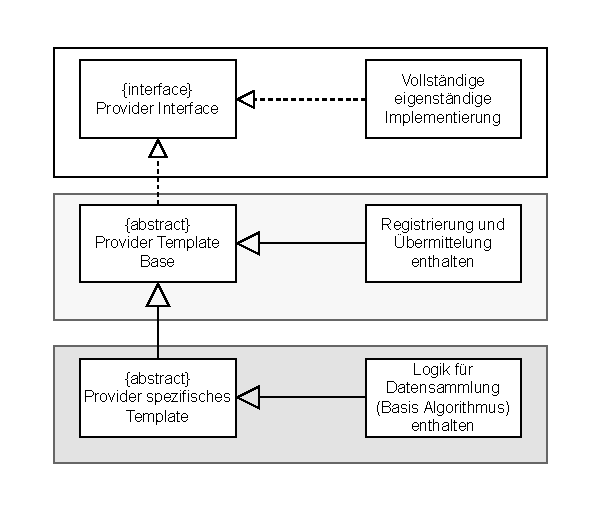
\includegraphics[width=0.52\textwidth]{5_Data_Provider_Structure}
\caption{Schema für Datenprovider.}
\label{fig:structure_data_provider}
\end{figure}

Wie in Abbildung \ref{fig:structure_data_provider} dargestellt, besteht die Möglichkeit, eigene Implementierungen von Providern zu erstellen. Dennoch wird empfohlen, mindestens den zweiten Layer des Frameworks zu verwenden. Die Basisimplementierung übernimmt bereits die Fehlerbehandlung und das Exception Handling, wodurch mögliche Fehlersituationen automatisch abgefangen werden.

Für den ersten Layer hingegen sind detaillierte Kenntnisse über den Tracking Manager erforderlich, da in dieser Ebene die Registrierung der Provider manuell erfolgen muss.

Für die Standard-Provider sollten daher unbedingt die bereitgestellten Templates verwendet werden, da diese ausreichende Flexibilität bieten und gleichzeitig eine robuste sowie einheitliche Implementierung sicherstellen.

\section{Filterung und Extraktion}
\label{sec:data_extraction_concept}
Wie bereits im Unterabschnitt \ref{subsec:data_collection_components} beschrieben, werden die Daten während der Sammlung nach dem Push-Prinzip weitergegeben, ohne dass zuvor eine Filterung oder Aggregation erfolgt. Dieses Vorgehen hat Performance-Vorteile, da die Übertragungszeit in der Regel kürzer ist als die Zeit, die für eine Filterung benötigt würde. Daher muss die Filterung in eine asynchrone Umgebung ausgelagert werden. Genau diese Umgebung wird in diesem Abschnitt beschrieben.

\subsection{Komponentenstruktur und Aufgabenverteilung}
In Abbildung \ref{fig:structure_data_processing} wird die Struktur der Filter- und Extraktionskomponente veranschaulicht.
Diese Komponente besteht im Wesentlichen aus einer Verarbeitungskette und einem Manager, der wie auch bei anderen Systemkomponenten, die Verwaltung der Komponente übernimmt. Die Datenverarbeitung erfolgt innerhalb der Verarbeitungskette: Die eingehenden Daten werden gefiltert, extrahiert und anschließend, abhängig von den ermittelten Ergebnissen, gegebenenfalls aggregiert. Ein vergleichbares Vorgehen findet sich beispielsweise in OpenTelemetry (siehe Unterabschnitt \ref{subsec:open_telemetry}), wo diese Aufgaben im Collector ausgeführt werden. Welcher Bestandteil der Komponente welchen Beitrag zur Gesamtfunktion leistet, wird im Folgenden näher beschrieben.

\begin{figure}[H]
\centering
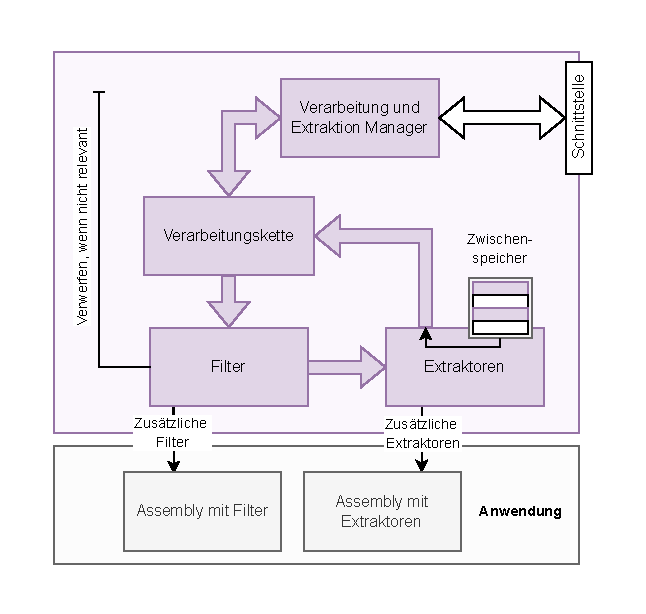
\includegraphics[width=0.6\textwidth]{5_Data_Processing_Structure}
\caption{Struktur Datenverarbeitungskomponente.}
\label{fig:structure_data_processing}
\end{figure}

\subsubsection{Manager für Verarbeitung und Extraktion}
Der Manager übernimmt, wie bereits bei den anderen Managern erwähnt, die Kommunikation mit dem übergeordneten Hauptmanager. Zusätzlich ermittelt er die Filter und Extraktoren und erzeugt die Verarbeitungskette. Er nimmt Daten asynchron entgegen und leitet diese an die Verarbeitungskette weiter. Ebenso erhält die Filterkette Extraktionsaufträge und leitet diese an die Verarbeitungskette weiter. Werden die Daten vom Hauptmanager angefordert, übergibt der Manager die extrahierten Daten aus der Verarbeitungskette. Die Hauptaufgabe des Managers liegt somit in der Datenvermittlung und der Steuerung der Verarbeitungskette, wie in Abbildung \ref{fig:structure_data_processing} veranschaulicht.

\subsubsection{Verarbeitungskette}
Die Verarbeitungskette umfasst die Filter und Extraktoren und steuert deren Initialisierung sowie Ausführung. Die Filterkette entscheidet dabei, welche Filter in welcher Reihenfolge ausgeführt werden. Die Initialisierung erfolgt primär anhand der Extraktionsaufträge, die jeder Extraktor berücksichtigen muss, um die exakt konfigurierte Datenmenge zu erhalten. Die Verarbeitungskette ist austauschbar, z.B. wenn die Strategie für die Ausführungsreihenfolge geändert werden soll.

\subsubsection{Filter}
Filter folgen einem bestimmten Schema und entscheiden, ob Daten weiterverarbeitet werden. Dies ist beispielsweise sinnvoll, wenn bestimmte Aktionen mehrfach hintereinander auftreten, aber die gleiche Bedeutung haben. Mit einem Filter können nachfolgende Aktionen für eine bestimmte Zeitspanne blockiert werden. Die eingehenden Daten, z.B. Aktionen oder sonstige Informationen, werden bei einem negativen Prüfung verworfen und an die Speicherverwaltung übergeben (siehe Abbildung \ref{fig:structure_data_processing}).

\subsubsection{Extraktoren}
Extraktoren verarbeiten Daten (Aktionen und sonstige Informationen) basierend auf den Extraktionsaufträgen. Dabei werden die Daten, die nach dem Push-Prinzip übertragen werden, genau auf die Konfiguration zugeschnitten, sodass nur relevante Daten im Ergebnis verbleiben. Die extrahierten Daten werden, wie in Unterabschnitt \ref{subsec:extraction_data_and_converting} beschrieben, weiter aggregiert und in bestimmten Objekten in vorgegebener Form abgelegt.

Um eine schnelle Aggregation und Datenübertragung bei Abruf zu gewährleisten, werden die Daten pro Extraktor gespeichert, kontinuierlich bearbeitet und im Arbeitsspeicher gehalten (siehe Abbildung \ref{fig:structure_data_processing}). Die Speicherung erfolgt im Hauptspeicher und wird nach Programmende oder durch den Garbage Collector freigegeben. Da die Daten nicht zu den primären Anwendungskomponenten gehören, können so Fehler durch externe Speicherung vermieden werden und ein Verlust der Daten hat keine Bedeutung.

\subsection{Extrahierte Daten und Weiterverarbeitung}
\label{subsec:extraction_data_and_converting}
Im Unterabschnitt \ref{subsec:communication_between_coponents} wurde beschrieben, dass die Extraktionsdaten als Kommunikationsobjekte fungieren. Genau diese Objekte werden in diesem Teil der Anwendung von den Extraktoren erzeugt. 

\subsubsection{Inhalte der Datenobjekte}
Betrachtet man die vollständige Konfiguration, so ergeben sich Objekte mit folgendem Inhalt:

\begin{itemize}
    \item \textbf{Workflow-Daten:} Enthalten den Ablauf eines Workflows als String, abgeleitet aus den Metainformationen des Extraktionsauftrags, sowie die Anzahl der Abläufe eines solchen Workflows.
    
    \item \textbf{Automatische Workflow-Daten:} Beinhalten die Aktionen innerhalb einer Ansicht, die in einem bestimmten Zeitraum in einer definierten Reihenfolge auftreten. Diese Daten dienen der weiteren Auswertung.
    
    \item \textbf{Nutzungsdaten:} Diese sind weiter unterteilt und enthalten folgende Informationen:
    \begin{itemize}
        \item \textbf{Funktionsnutzung:} Beschreibt, wie oft eine bestimmte Funktionalität aufgerufen wurde und um welche Funktion es sich handelt.
        \item \textbf{Tastaturnutzung:} Beschreibt, wie Shortcuts innerhalb einer Ansicht verwendet wurden.
        \item \textbf{Steuerelementnutzung:} Beschreibt, welche Ereignisse eines Steuerelements wie häufig auftreten.
        \item \textbf{Benutzerdefinierte Aktionen:} Beschreibt eine benutzerdefinierte Aktion sowie deren Häufigkeit des Auftretens.
    \end{itemize}
    
    \item \textbf{Metriken:} Sind numerische Werte, die weiter in folgende Kategorien unterteilt werden:
    \begin{itemize}
        \item \textbf{Ladezeiten:} Stellen aggregierte Daten zu den Ladezeiten einer Ansicht dar.
        \item \textbf{Ansichtsnutzung:} Wie oft wird eine bestimmte Ansicht verwendet.
    \end{itemize}
    
    \item \textbf{Kontextinformationen:} Daten, die aus einer Ansicht oder einem \textit{PresentationModel} ausgelesen werden.
\end{itemize}

\subsubsection{Weiterverarbeitung der Datenobjekte}
Um Flexibilität zu gewährleisten, können die Daten vor der Übergabe in ein eigenes Format konvertiert werden. Dadurch ist es beispielsweise möglich, die Daten anschließend für Systeme wie Google Analytics (siehe Unterabschnitt \ref{subsec:google_analytics}) weiterzuverarbeiten. 

Die gewünschte Konvertierung muss in der Systemkonfiguration (siehe Abschnitt \ref{sec:integration_concept}) angegeben werden. Für das JSON-Format existiert bereits eine Implementierung, die vom Framework bereitgestellt wird.

\section{Systemkonfiguration}
\label{sec:integration_concept}
Das Framework benötigt bestimmte Informationen, wie bereits in den vorherigen Komponenten beschrieben wurde. Zudem soll das Framework unabhängig von den Services der Anwendung bleiben und diese nicht direkt referenzieren. Um diese lose Kopplung zur Anwendung zu gewährleisten, stellt die Anwendung eine Systemkonfiguration bereit (siehe Abbildung \ref{fig:structure_relationship_systemconfiguration}). Diese Konfiguration dient als Adapter zwischen Framework und Anwendung und leitet Aufrufe über Delegation an die Anwendung weiter. Die Anwendung entscheidet anschließend selbst, beispielsweise wo und wie Daten publiziert werden oder ob das Tracking überhaupt gestartet werden soll.

\begin{figure}[H]
\centering
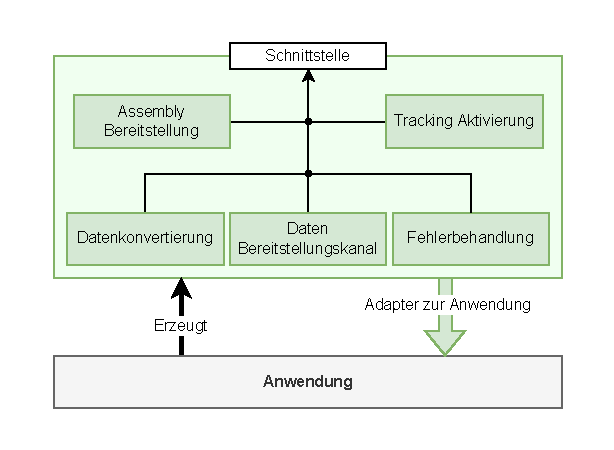
\includegraphics[width=0.53\textwidth]{5_Tracking_Systemkonfiguration}
\caption{Systemkonfiguration Aufbau und Beziehung zur Anwendung.}
\label{fig:structure_relationship_systemconfiguration}
\end{figure}




